\documentclass{article}
\title{Testing How Distance Can Change the Minimum Distance Needed to Perceive Change From a D400 Depth Camera}
\date{June\\19\\2019}
\author{Aaron Jencks\\Electronics Technology Technician Intern, JET Engineering}

\usepackage{pgfplots}

\usepackage{graphicx}
\usepackage{media9}

\usepackage{listings}

\usepackage{hyperref}
\hypersetup{
	colorlinks=true,
	linkcolor=blue,
	filecolor=magenta,
	urlcolor=cyan,
}

\begin{document}
	\maketitle
	\newpage
	
	\tableofcontents
	\newpage
	
	\section{Summary}
		This procedure tests the minimum distance between two equally sized objects needed in order for an Intel Realsense D400 depth camera to detect the change.  We used a long table and separated it into ten equal parts, then placed the camera at one end and took measurements at the ten locations.
	
	\section{Setup}
		\subsection{Materials}
			\begin{enumerate}
				\item Intel Realsense D435/D415 Depth Camera
				\item A long table, at least 5.5' in length
				\item A mounting bracket to hold the camera in place between runs.
				\item Some sort of material for marking the ten positions to measure at.
				\item Two equally sized object to measure the minimum depth distance with.
				\item Caliper to measure this minimum depth.
			\end{enumerate}
		\subsection{Our Setup}
			For our setup we used a D435 depth camera, Painter's tape to mark the positions, two childrens' blocks to measurement, and a ruler to move them. See Figure \ref{fig:setup} for an image of our setup.
			
			\begin{figure}[h]
				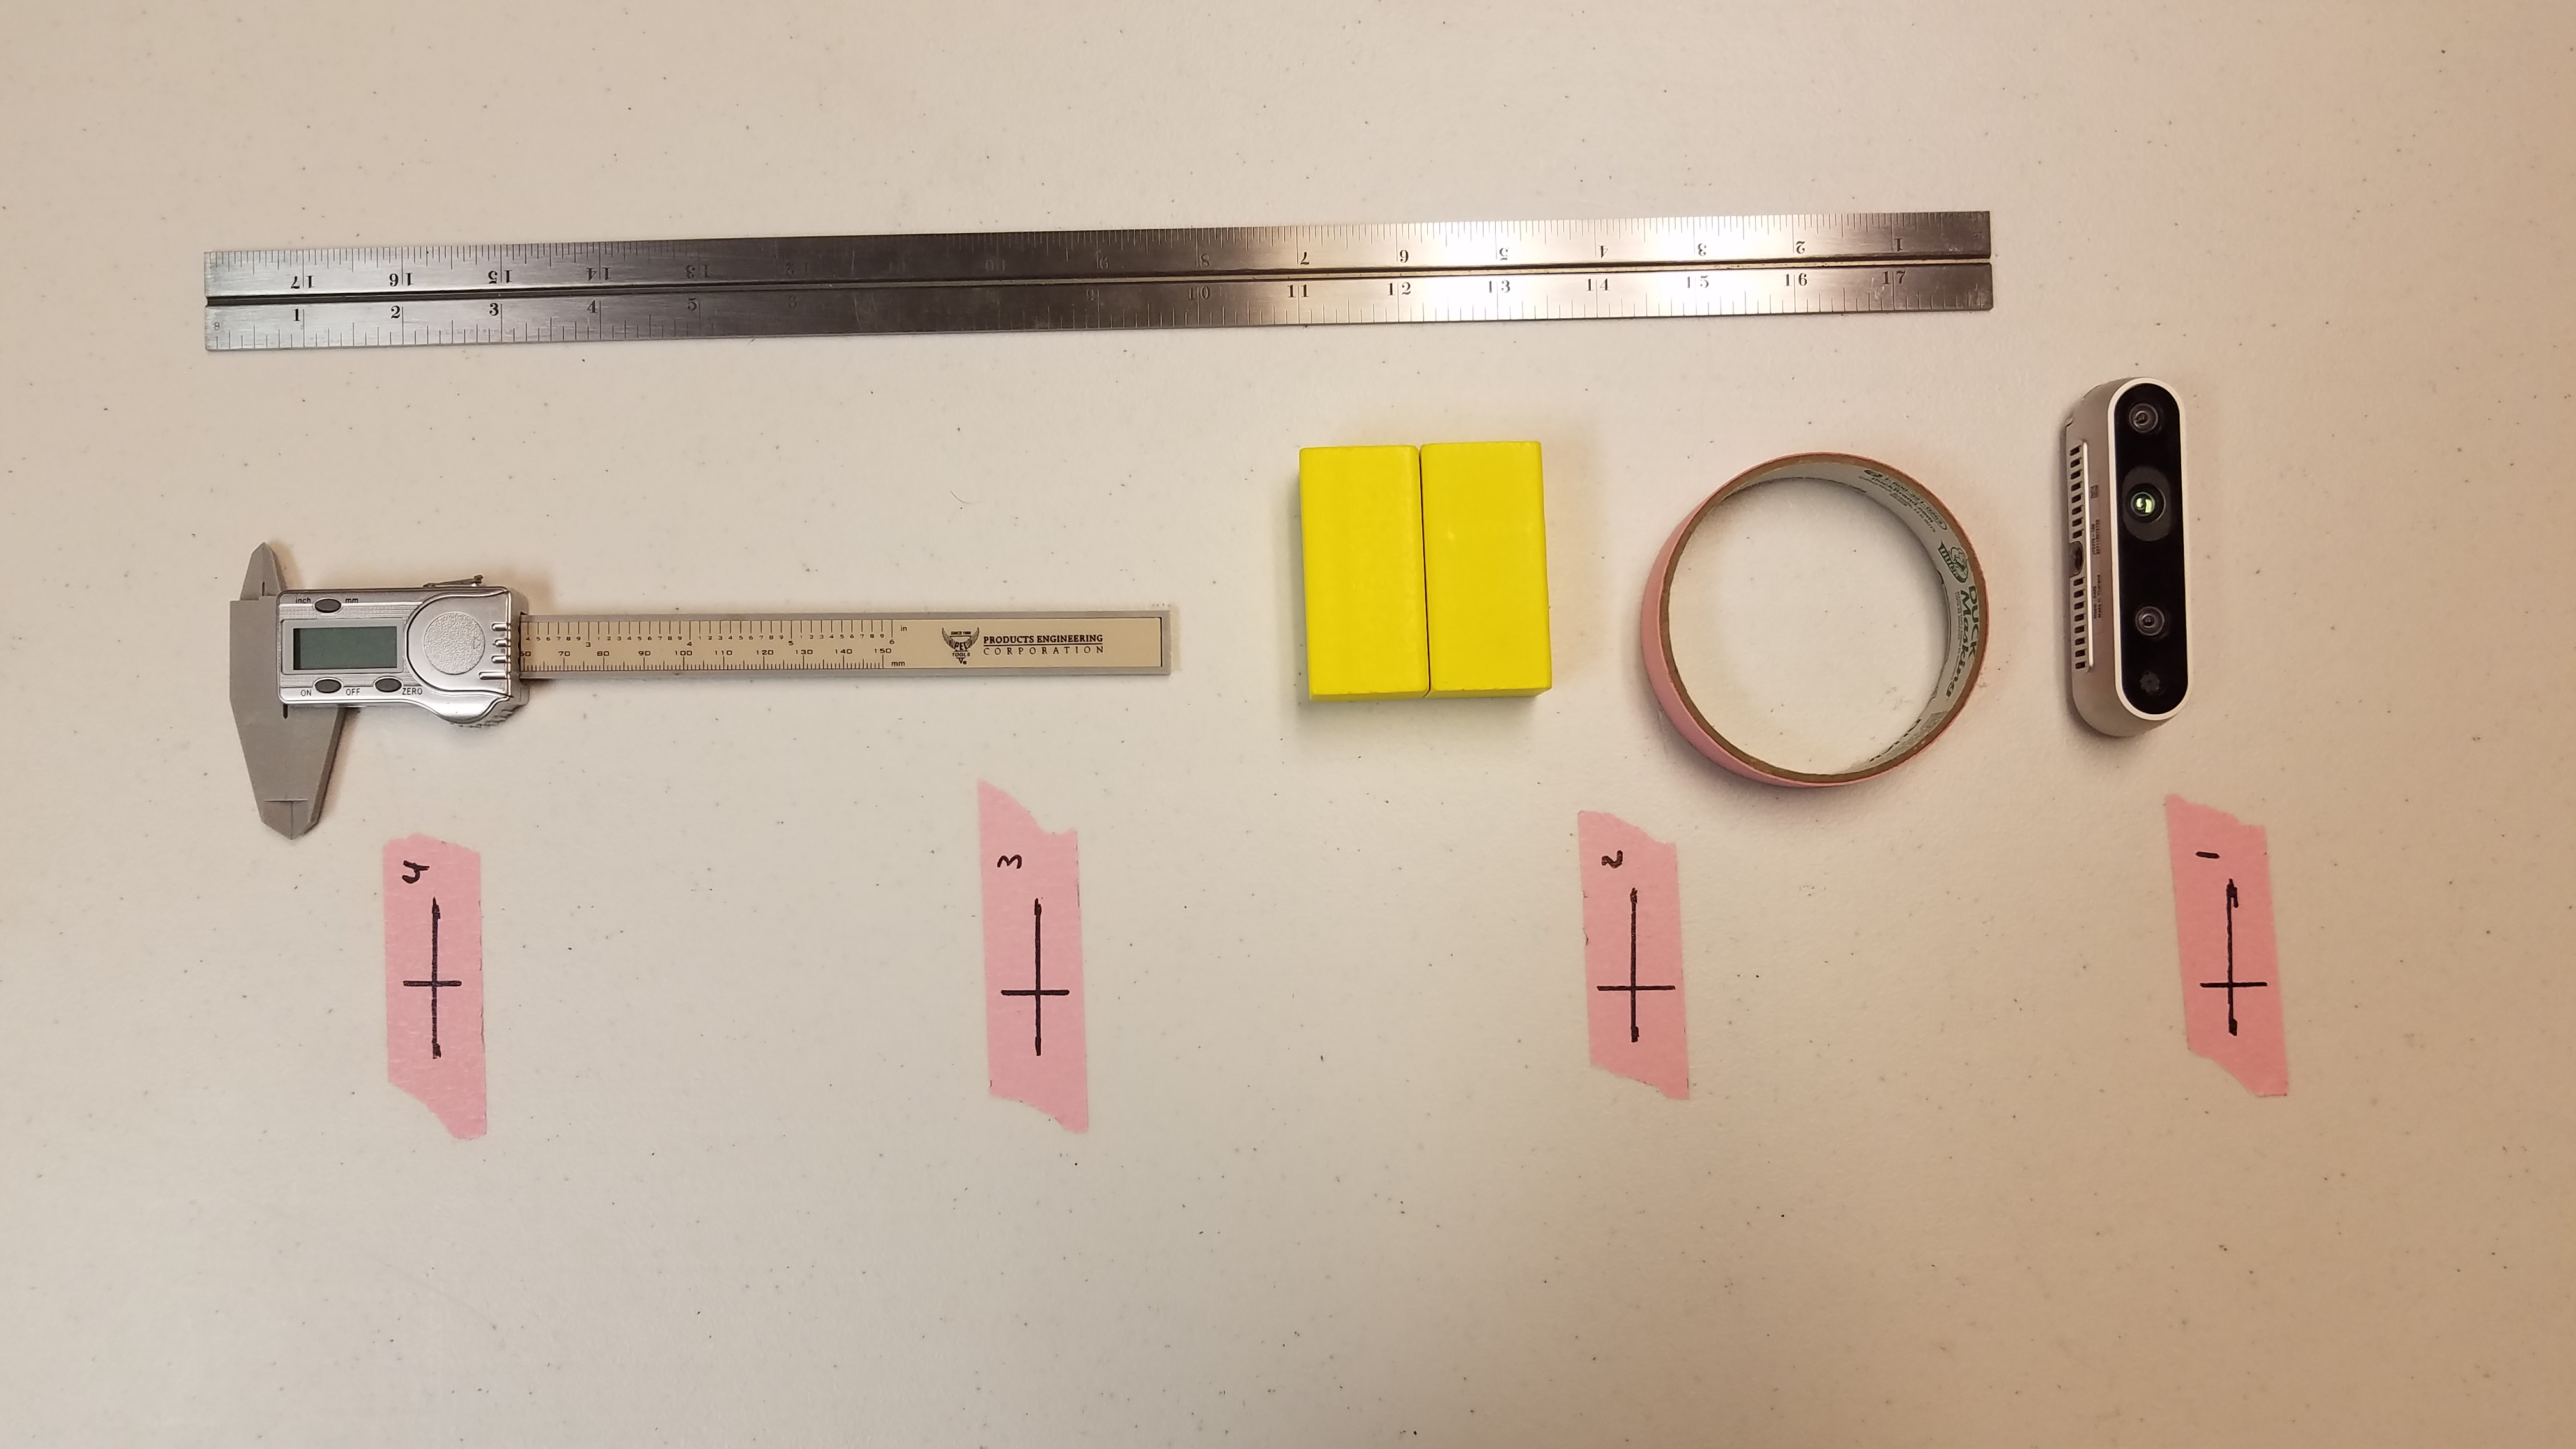
\includegraphics[width=8cm]{./images/our_setup.jpg}
				\centering
				\caption{Our setup}
				\label{fig:setup}
			\end{figure}
			
			\newpage
			We also used a custom mounting bracket, see Figure \ref{fig:bracket}.
			
			\begin{figure}[h]
				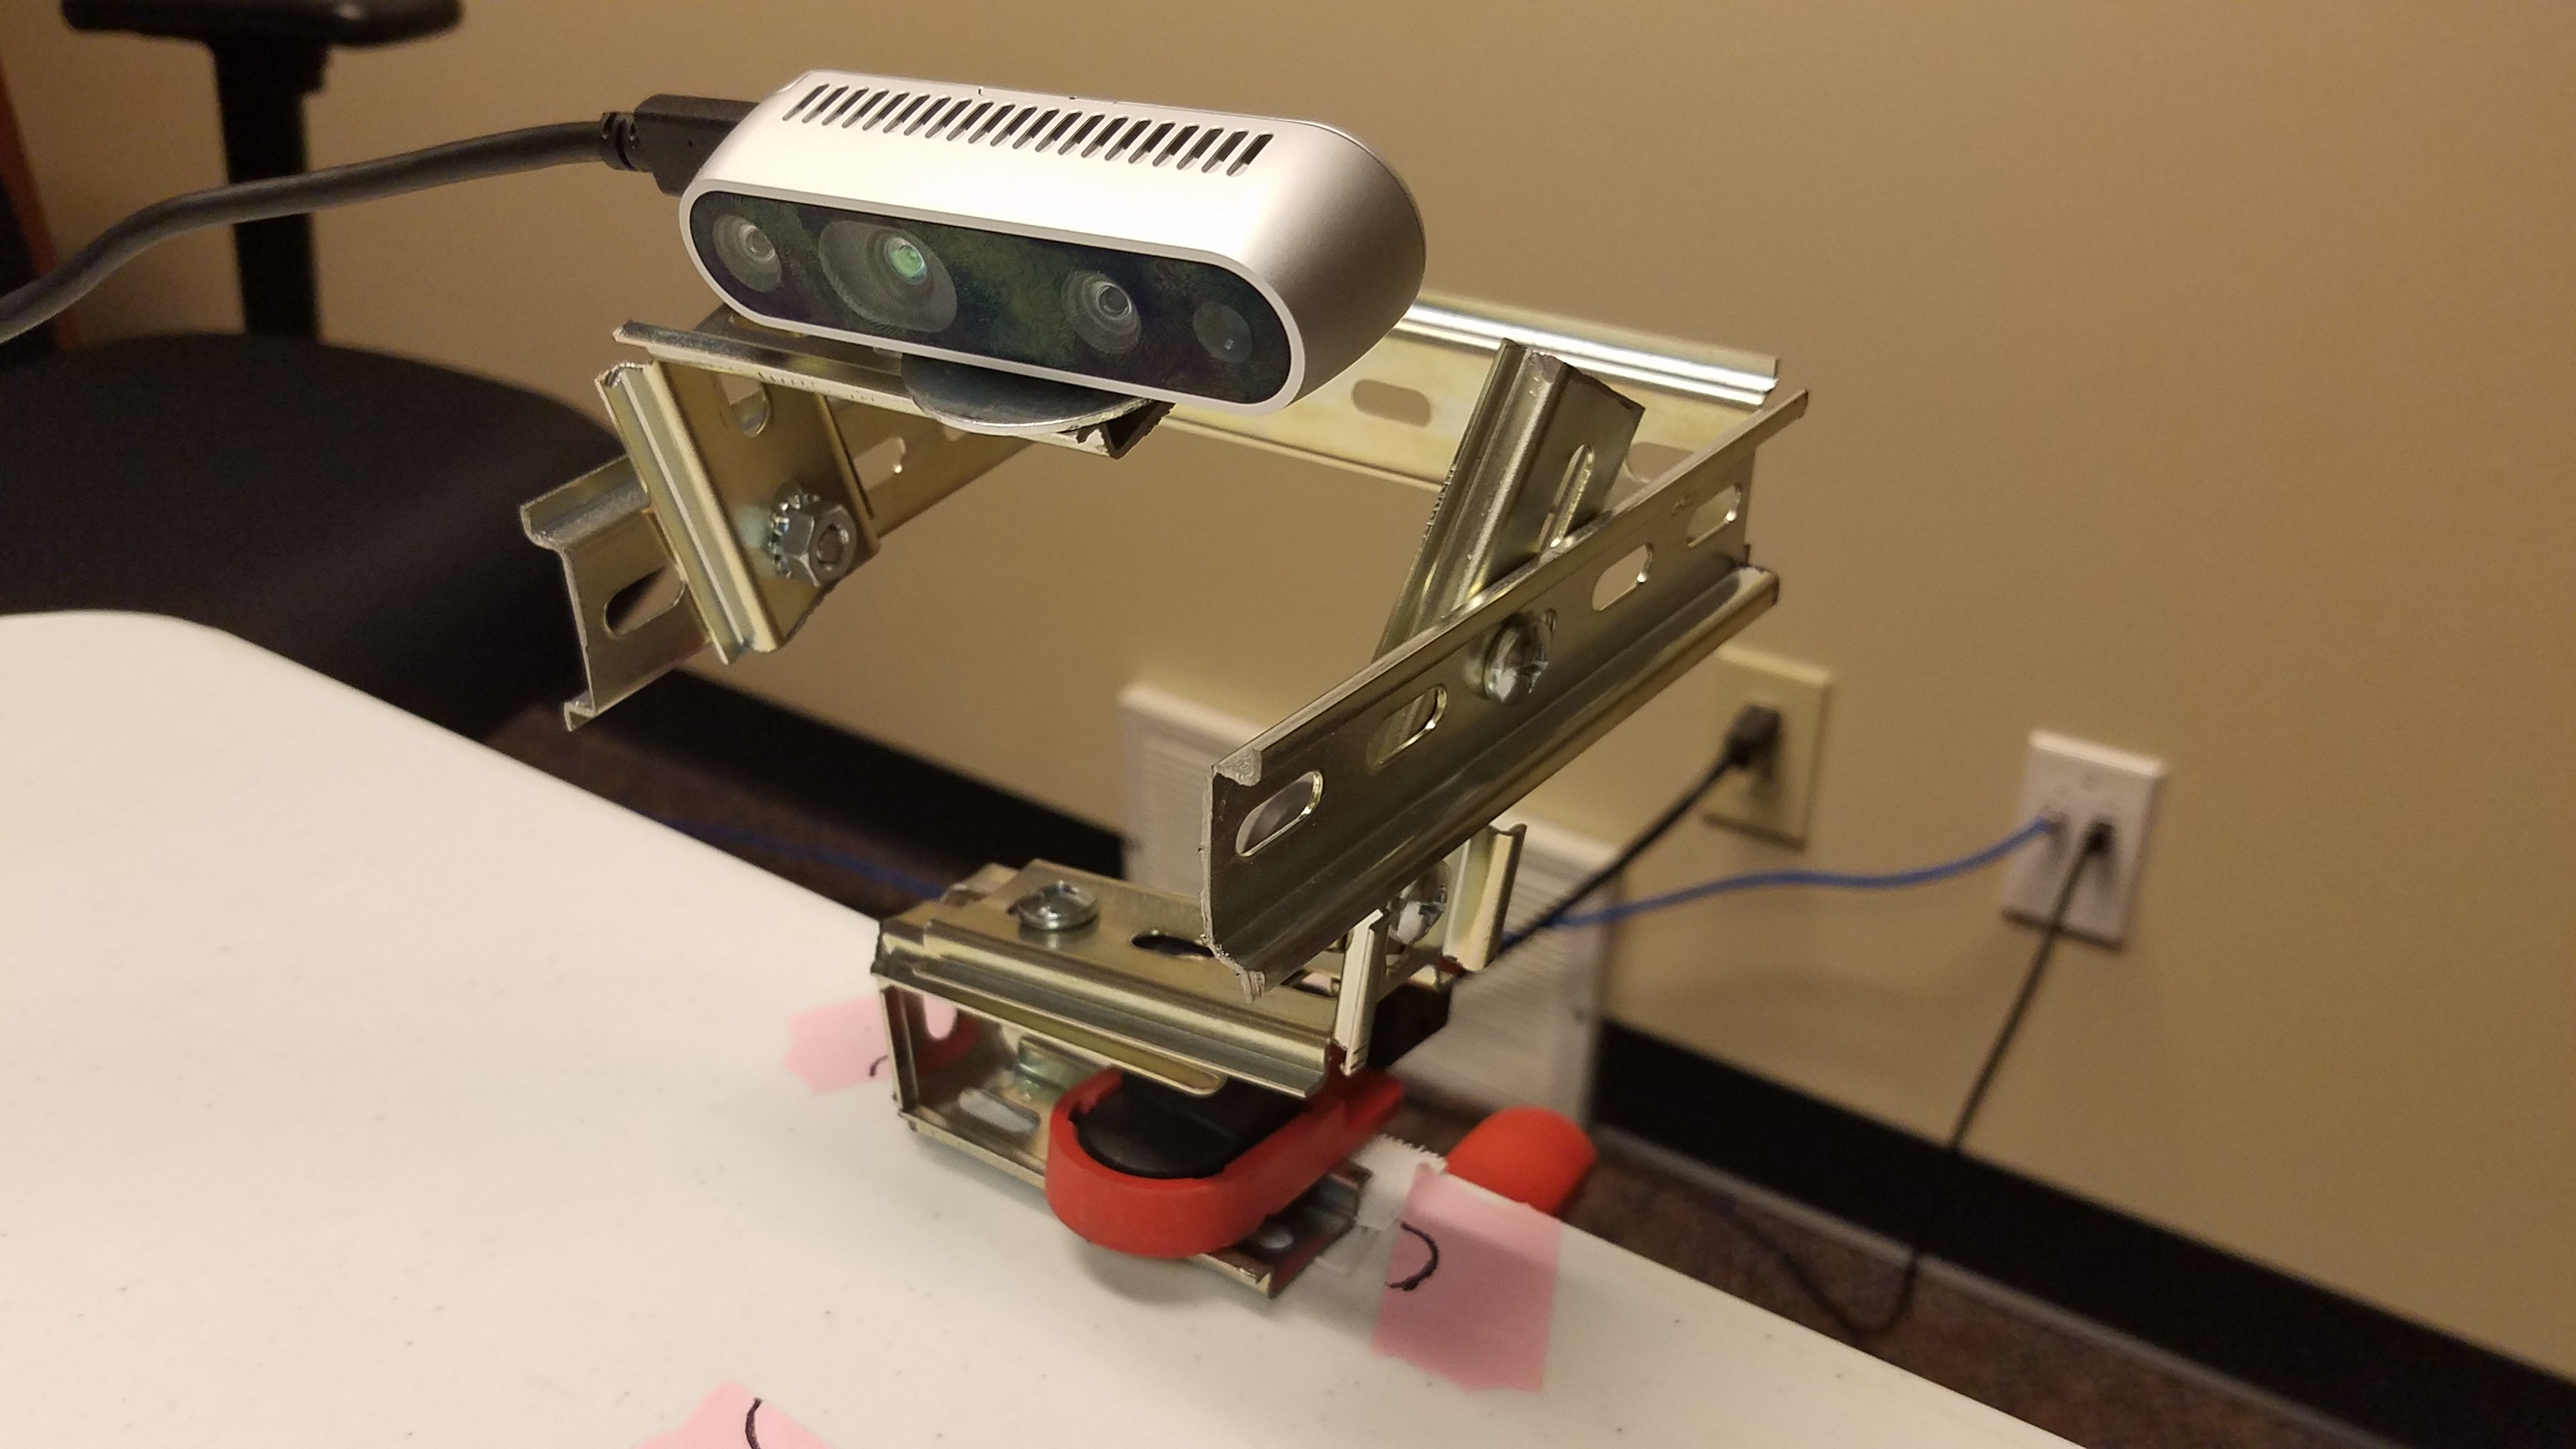
\includegraphics[width=8cm]{./images/mounting_bracket.jpg}
				\centering
				\caption{The Custom Mounting Bracket}
				\label{fig:bracket}
			\end{figure}
		
		\section{The Code}
			To stick with simplicity, instead of using the realsense's native SDK in C++, we used its python wrapper.  For this test, we used Python 3.6.8 with the following packages installed:
			\begin{itemize}
				\item pillow
				\item numpy
				\item matplotlib
				\item pyrealsense2
				\item cython
			\end{itemize}
			You can find a yml file \href{run:"../../Conda Environments"}{in the Conda Environments folder}.
			
			\newpage
			\subsection{Brief Code Description}
				This program is used to make data collection easier, it displays the data in a modulated way such that there are only two distinct colors on the screen, see Figure \ref{fig:codefrontexample}.
				
				\begin{figure}[h]
					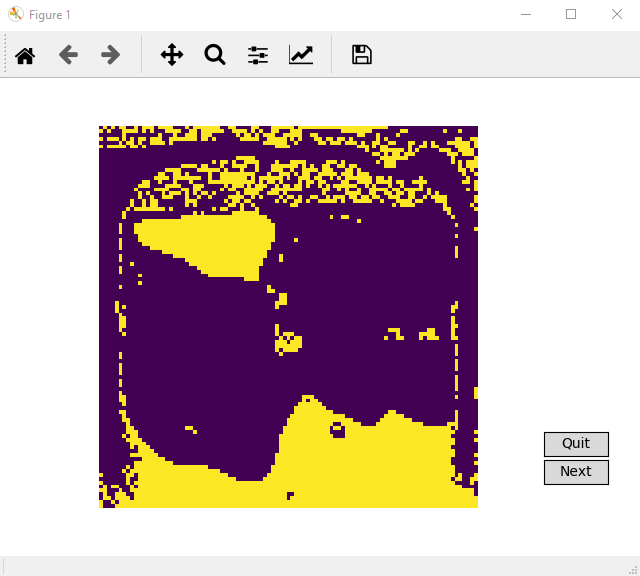
\includegraphics[width=8cm]{./images/code_display_example.png}
					\centering
					\caption{Code Front End}
					\label{fig:codefrontexample}
				\end{figure}
			
				\newpage
				\subsection{Static Settings}
					There is a variety of settings that can be adjusted manually before running the program
					
					\label{code:staticsettings}
					\begin{lstlisting}[language=Python]
cnf_file = "C:\\...\\realsense_cam_settings.json"
clumping = 1
depth_clumping = 1
historical_average_depth = 64

horizontal_trim = 0
vertical_trim = 0
rois = [
	{'l': 294, 'u': 262, 'r': 391, 'b': 360},  # Marker 1
	{'l': 312, 'u': 222, 'r': 378, 'b': 281},  # Marker 2
	{'l': 321, 'u': 198, 'r': 373, 'b': 243},  # Marker 3
	{'l': 325, 'u': 184, 'r': 369, 'b': 218},  # Marker 4
	{'l': 329, 'u': 175, 'r': 366, 'b': 201},  # Marker 5
	{'l': 321, 'u': 167, 'r': 366, 'b': 194},  # Marker 6
	{'l': 334, 'u': 162, 'r': 362, 'b': 190},  # Marker 7
	{'l': 335, 'u': 162, 'r': 359, 'b': 186},  # Marker 8
	{'l': 339, 'u': 159, 'r': 361, 'b': 179},  # Marker 9
	{'l': 341, 'u': 154, 'r': 360, 'b': 173}   # Marker 10
]
					\end{lstlisting}
					
					\subsubsection{cnf\_file}
						This points to the json file containing the settings for the camera, these can be set from the RealsenseViewer program.
						
					\newpage
					\subsubsection{clumping}
						This causes the program to average blocks of pixels together, see the following figures for examples
						
						\begin{figure}[h]
							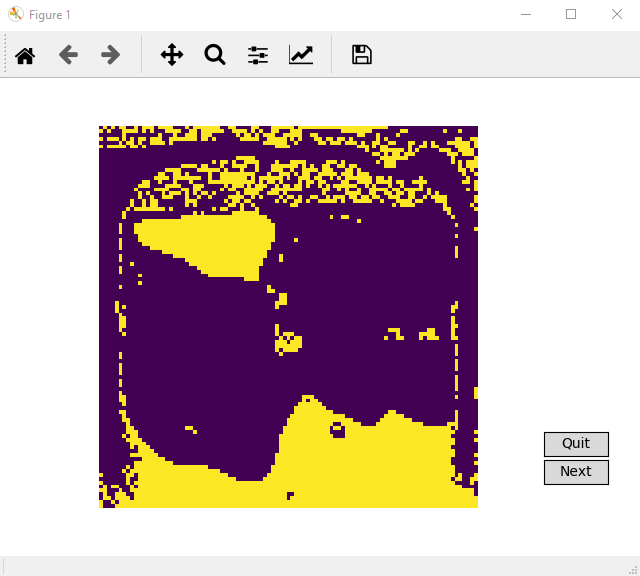
\includegraphics[width=4cm]{./images/code_display_example.png}
							\centering
							\caption{clumping = 1}
							\label{fig:clumpingexample1}
						\end{figure}
					
						The figure above shows with no clumping, the below example shows what happens when clumping is set to 3.
					
						\begin{figure}[h]
							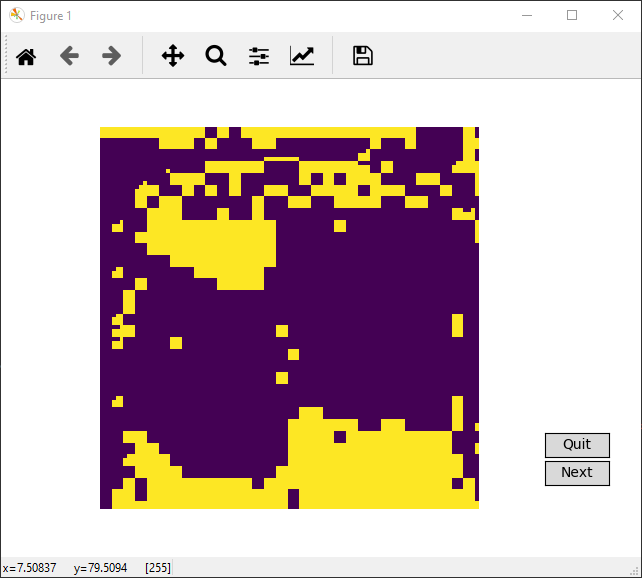
\includegraphics[width=4cm]{./images/code_clumping_example.png}
							\centering
							\caption{clumping = 3}
							\label{fig:clumpingexample3}
						\end{figure}
					
					\subsubsection{depth\_clumping}
						This determines how the 16-bit depth values are clumped together, a value of 1 means that there is no clumping, a value of 100, for example would take every 100 values and clump them into 1 value (ie. 6500-6599 would become 65, before being modulated.)
						
					\subsubsection{historical\_average\_depth}
						This number determines how many frames are kept in a history buffer and then averaged together, pixel-by-pixel (ie. With a value of 64, pixel 105x105 is averaged with the last 64 values for 105x105).
						
					\subsubsection{horizontal\_trim}
						This number shifts the camera \hypertarget{roi}{Region Of Interest (roi)} horizontally to the right by n where n is the value of horizontal\_trim.
						
					\subsubsection{vertical\_trim}
						This number shifts the camera \hyperlink{roi}{roi} vertically downwards by n where n is the value of vertical\_trim.
						
					\subsubsection{rois}
						This list specifies the regions, in pixels, where the camera should be looking for each of the 10 locations. The letters stand for the following:
						\begin{itemize}
							\item l: left
							\item r: right
							\item u: upper
							\item b: bottom
						\end{itemize}
						Each line in the list corresponds to the next section, they are marked with a comment denoting the location number right next to it, see the code listed at \ref{code:staticsettings}.
						
				\subsection{Description of Operation}
					How the code operates is that it streams video from the camera, then takes the data after it has been clumped together using the above settings (see \ref{code:staticsettings}) and modulates it for odd and even numbers, odd numbers are yellow and even numbers are purple. This is then displayed to the screen, you can use the 'next' button to move onto the next location \hyperlink{roi}{roi}. Use the 'quit' button to exit the program, do not use the 'X' button, it breaks the software.
					
			\newpage
			\section{Process}
				This section will explain how to reproduce the experiment.
				\subsection{Setup}
					Place the camera on the mount and mark the 10 locations you would like to test. See the image below.
					
					\begin{figure}[h]
						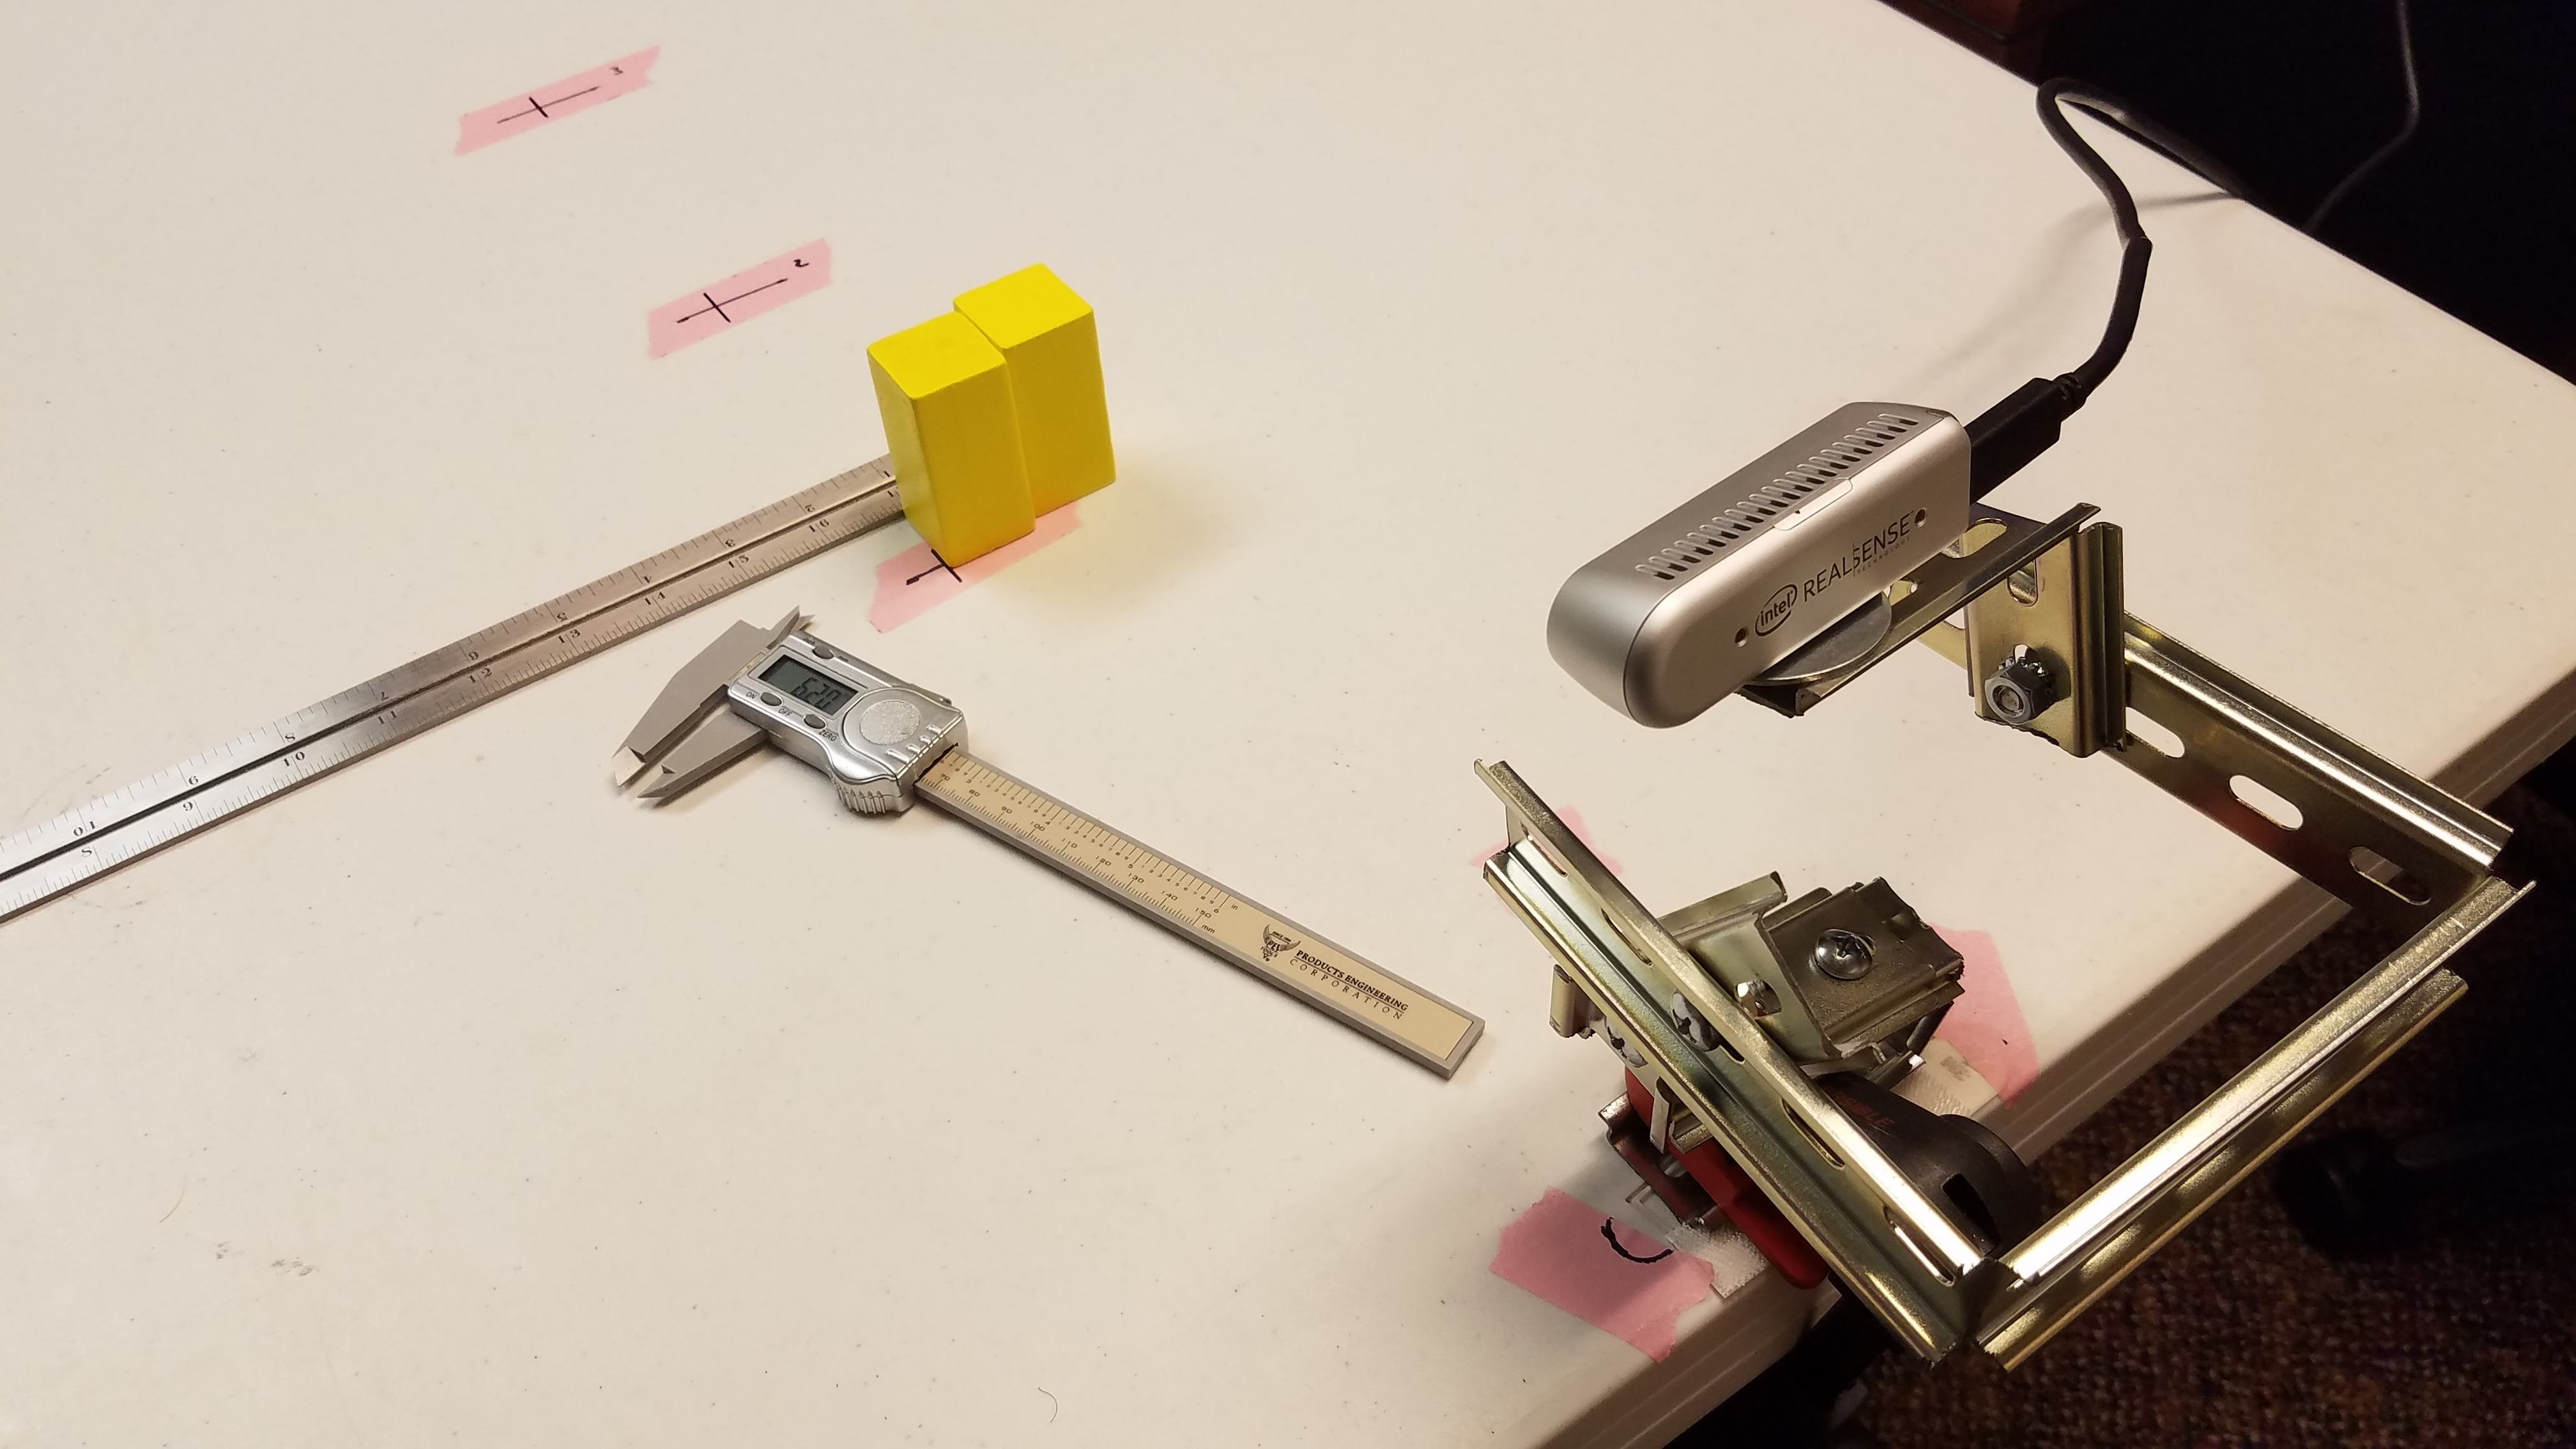
\includegraphics[width=8cm]{./images/initial_setup.jpg}
						\centering
						\caption{Initial Testing Setup}
						\label{fig:initsetup}
					\end{figure}
				
					Align the objects so that the front of the objects are perfectly flat facing the camera. Run main.py from the Depth Displayer the console will tell you that you are on location 1. See Figure \ref{fig:consoleinit}.
					
					\begin{figure}[h]
						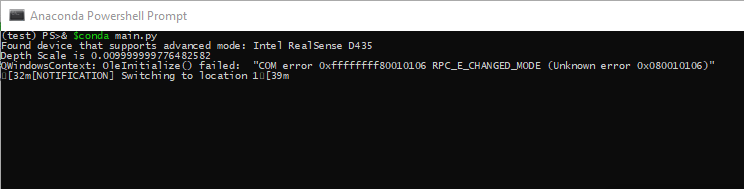
\includegraphics[width=8cm]{./images/code_initial_console_output.png}
						\centering
						\caption{Initial Software Output}
						\label{fig:consoleinit}
					\end{figure}
				
					\newpage
					Slowly move one of the objects forward until you see a pixel shift on one of the blocks in the display. If you are moving towards the camera, you should note a downward shift on the display, and if you are moving away from the camera, you should note a upward shift on the display. For example measurement, see Figure \ref{fig:examplemeasvideo}.
					
					\begin{figure}[h]
						\includemedia[width=8cm,activate=pageopen,addresource=./videos/measurement_example_edit.mp4,
						flashvars={source=./videos/measurement_example_edit.mp4}]{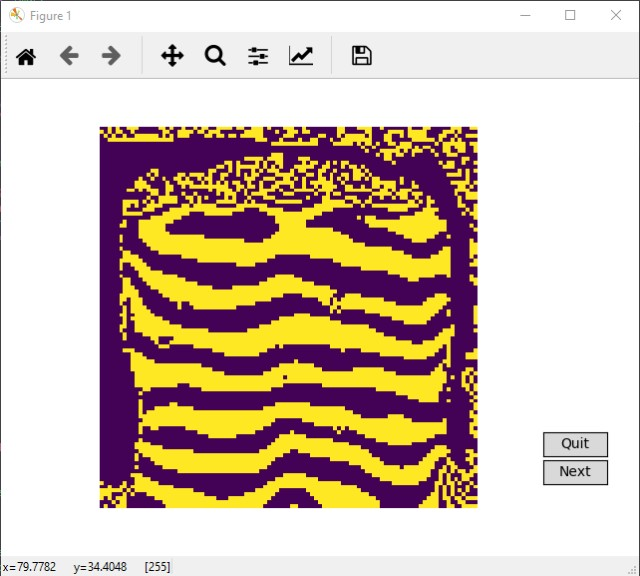
\includegraphics[width=8cm]{./videos/measurement_example_Moment.jpg}}{VPlayer.swf}
						\centering
						\caption{Example of the Measurement Process}
						\label{fig:examplemeasvideo}
					\end{figure}
				
					When the block moves forward, you can see the stripes start moving downwards, this is a change in depth value.
					
					Once you've moved the block, and the stripes move, then measure the distance between the two objects with the caliper and write that down, then repeat, moving the objects back to the next location and clicking the 'next' button on the display.
					
				\newpage
				\section{Results}
					We did the measurements with 3 different depth scales, 5 trials per, 0.0001, 0.001, and 0.01.
					
					\subsection{Depth Scale 0.0001}
						\begin{figure}[h]
							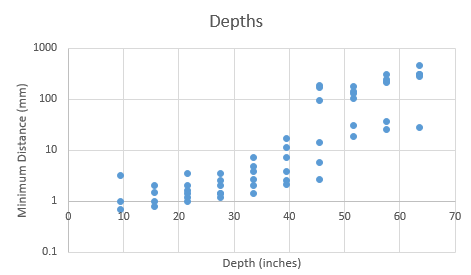
\includegraphics[width=8cm]{./images/DS_0001.png}
							\centering
							\caption{Data for Depth Scale 0.0001}
							\label{fig:ds0.0001}
						\end{figure}
					
					\subsection{Depth Scale 0.001}
						\begin{figure}[h]
							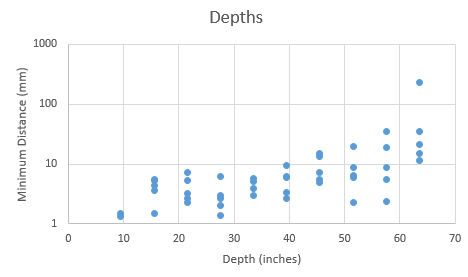
\includegraphics[width=8cm]{./images/DS_001.png}
							\centering
							\caption{Data for Depth Scale 0.0001}
							\label{fig:ds0.0001}
						\end{figure}
					
					\newpage
					\subsection{Depth Scale 0.01}
						\begin{figure}[h]
							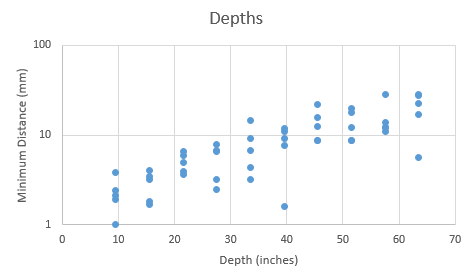
\includegraphics[width=8cm]{./images/DS_01.png}
							\centering
							\caption{Data for Depth Scale 0.0001}
							\label{fig:ds0.0001}
						\end{figure}
					
					\subsection{Discussion}
						From the results above I've concluded that the intel realsense depth cameras must have some sort of critical range, similar to a transistor with a linear region from the min$_z$ to about 4-5 feet, at which point the perception exponentially declines. But this characteristic seems to be inversely proportional to the actual depth scale, so the larger the depth scale (ie 0.01) the better the linearity of the perception, but this might be due to the limited range of the experiment, so with a longer table, it might prove that the 0.01 trial might actually have an exponential curve as well, it's just farther than length of the table.
			
		\newpage
		
		\listoffigures
	
\end{document}